\documentclass[12pt]{article}
\usepackage{amsmath,amssymb}
\textheight 240mm
\textwidth  170mm
\oddsidemargin  0mm
\evensidemargin 0mm
\topmargin -20mm

\usepackage[utf8]{inputenc}
\usepackage{graphicx}
\usepackage{float}
\usepackage{titling}
\usepackage{geometry}
\usepackage{color}

\geometry{ a4paper,
	left=30mm,
	right=30mm,
	top=20mm,
}

\addtolength{\headheight}{0.2pt}
%\setlength{\droptitle}{-8em}

\title{Music Genre Classification}
\author{Abhijit Suresh, Paria Rezaeinia, Sahana Sadogopan}

\begin{document}
	\maketitle

\section{INTRODUCTION}
Music genre classification is the task of classifying the given audio signal into its corresponding categorical description (a.k.a. genre). It is a very challenging task in the field of music information retrieval (MIR) and widely used for digital music service and Internet radio. For example: music applications such as Shazam identify a song based on its audio content. The goal of this project is to design a classifier that takes audio signal as input and produces its corresponding genre as the output.

The data set we are using for this project is from the website of the 5th International Conference on Music Information Retrieval (ISMIR2004), and it is available in Pulse Coded Modulation (PCM). There are a total of 729 songs. The number of songs in each genre is as follows:
\begin{itemize}
	\item Classical: 320 songs
	\item Electronics: 115 songs
	\item Jazz-blues: 26 songs
	\item Metal-punk: 45 songs
	\item Rock-pop: 101 songs
	\item World: 122 songs
\end{itemize}
The objective is to train a classifier on this data that can classify any song into these 6 different genres. We have explored and experimented with several approaches to this problem. In order to train and test data, we use 10-fold cross validation (i.e, 90\% of the songs are being used for training  and 10\% of the songs for testing).

Our approach to this problem consists of 3 main components; dimensionality reduction, quantifying the distance between two songs in the reduce spaced and statistical learning. The organization of the paper is as follows: dimensionality reduction techniques are discussed in section \ref{dr} followed by section \ref{sec:dist} which explores the different distance metrics and section \ref{sec:stat} which explains the statistical learning methods we have used to classify the data. In section \ref{sec:exp} we represent the results of our approach and finally in section \ref{sec:disc} we talk about the results and future work.

\section{DIMENSIONALITY REDUCTION}\label{dr}
%_________________________________________________________________
As the first step, we need to sample the songs in order to analyze and train the data. After the sampling of the given data set, we extract features or coefficients from the sampled space. However, the number of features are represented as a point in high dimensional space. When the dimension is enormously huge, the data becomes sparse as the volume increase. This is known as the curse for dimensionality. Hence, in order to classify the data we need to reduce the number of dimensions.Once the dimensionality is reduced, we can use different classification methods.

In order to tackle the curse of dimensionality, we used Johnson-Lindenstrauss lemma to decide the minimum number of dimensions. The idea behind Johnson-Lindenstrauss lemma is that points in high-dimensional space can be projected onto low dimensional space while preserving the distance between the points \cite{dasgupta}. For a given dataset, the minimum number of dimension required to preserve the distance between the points is given by the formula $$ n > 8 * ln(m) * \epsilon ^ 2 $$ where $\epsion$ is a number between 0 and 1. For this project we have $$ n > 77$$ and hence the number of cepstrum coefficients that we have considered is 79.
%_________________________________________________________________
\subsection{MFCC(MEL FREQUENCY CEPSTRUM COEFFICIENT) }
One of the dimensionality reduction techniques that we were interested in is MFCC (Mel Frequency Cepstrum Coefficient) \cite{logmfcc}. In Mel Frequency Cepstrum, the frequency bands are equally spaced in mel space which is approximated by the human auditory system clearly and hence this frequency system allows for better representation of song.
The MFCC coefficient follows a sequence of steps through which the coefficients are found.
The diagram below shows the sequence of steps in the generation of the MFCC coefficient.
\begin{figure}[H]
\center
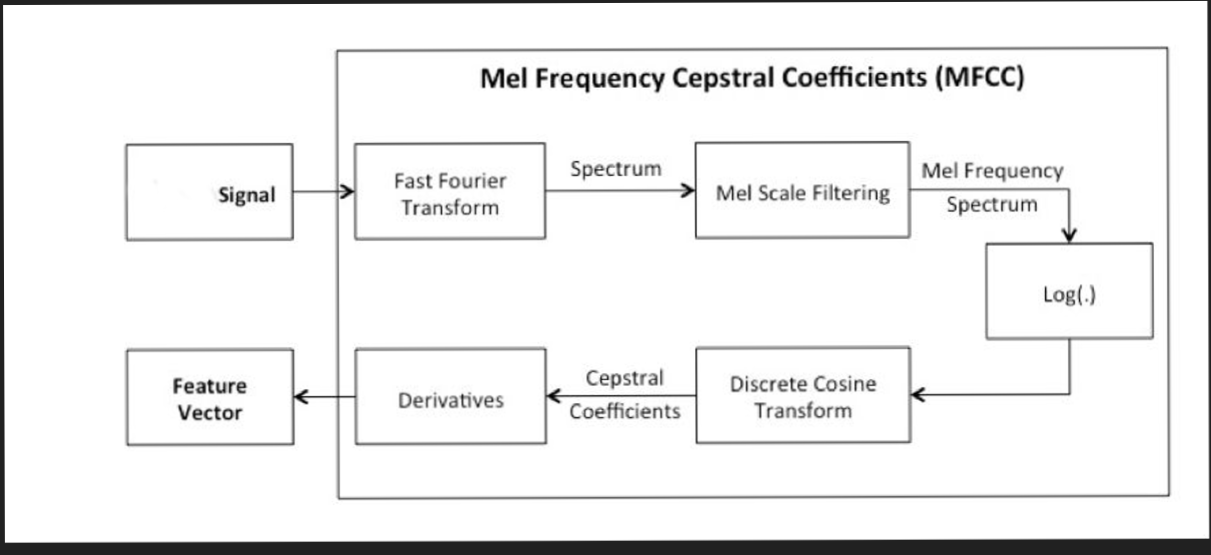
\includegraphics [scale=0.5]{mfcc.png}
\caption{mfcc algorithm}
\end{figure}
Based on the algorithm, after the signal is sampled ,  the Fourier transformation is performed and the spectrum obtained is passed through the Mel Scale Filter. The output that we obtain is in the Mel Frequency spectrum.
The log of the result is taken and a discrete cosine transform is applied to the signal in order to obtain the Mel Frequency Coefficient.
After performing the MFCC we have the signal separated into different frames and each frame contains a set of feature vectors. Based on Johnson Lindenstrauss we have identified 79 coefficients per frame.The number of frames changes based on the length of the song.
\subsection{PCA}
PCA(Principal Component Analysis) is a linear transformation technique which can be used to perform dimensionality reduction. PCA reduces the dimension by projecting the d dimensional data set onto k dimensional subspace where $k<d$ \cite{holand}. The data that we obtained from MFCC is taken as the input to  PCA. This has been done as an effort to reduce the dimension further.The principal components are identified based on the variance of the data. The first principal component has the maximum variance.The algorithm is as follows:
\begin{itemize}
  \item The data obtained from MFCC is normalised first
  \item The mean of the normalised data is put in a matrix and the mean value for all the rows are obtained.
  \item The variance of the data from MFCC is calculated.
  \item The Eigen values and Eigen vectors are calculated from the covariance matrix.
  \item The Eigen vectors are sorted in descending order in order to get the k largest eigen values.A new matrix is formed from the dominant eigen values.
  \item Then the data set is project on this new subspace and the feature vector are organised.
\end{itemize}
\subsection{CONTENT BASED SIMILARITY}
Beth and Ariel \cite{logan} presents a novel approach to compare songs based on their corresponding audio content. For each song in the dataset, they create a song signature. The song signature is generated based on k-means clustering of spectral features. The algorithm is summarized in figure (\ref{content}) below.

\begin{figure}[h]\label{content}
\center
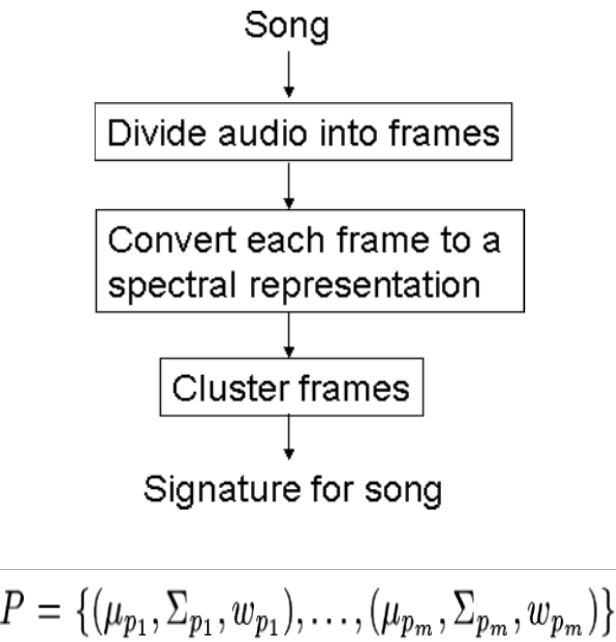
\includegraphics{fig1.png}
\caption{Content based similarity method}
\end{figure}

The first step is to divide the audio into multiple frames. Then, each frame is converted into its corresponding spectral representation. In order to generate the spectral representation we made use of MFCC algorithm which is explained in the previous sub section. The number of cepstrum coefficients was calculated based on the Johnson-Lindenstrauss lemma (n=79).

\subsubsection{K-MEANS}
Once each frame is transformed into its corresponding spectral representation, we cluster the frames using unsupervised k-Means clustering algorithm where the value of k is fixed to 10. k-Means is a popular clustering algorithm used in data mining. It is often confused with k-nearest neighbour algorithm. Given a set of n observations in a d dimensional space, k-Means aims to cluster the n dimension into k sets $S = {S_1,S_2,...S_k}$ where $ k \leq n$. The idea is to find the sum of distance functions of each point in the cluster to the K center. The equation is given by (\ref{kmeans}):

\begin{figure}[h]\label{kmeans}
\center
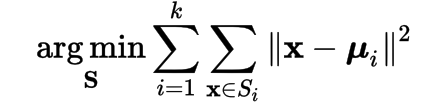
\includegraphics[scale=0.8]{fig2.png}
\caption{k-Means}
\end{figure}

\paragraph{}
After identifying the clusters, the mean, covariance and weight is calculated for each cluster. This set of values forms the signature of the song. This signature is used in order to compare two songs.

\subsection{MIXTURE MODEL}
Mixture model is a probabilistic model used in statistics in order to identify the sub-components of a probability distribution. The Gaussian mixture model (GMM) is a special case of mixture model with Gaussian sub-components. The intuition behind the mixture model is that the underlying components represent the set of hidden classes within the system. The following figure is a good representation of the Gaussian mixture model which represents the Gaussian components of a probability distribution.
\begin{figure}[H]\label{GMM}
	\centering
	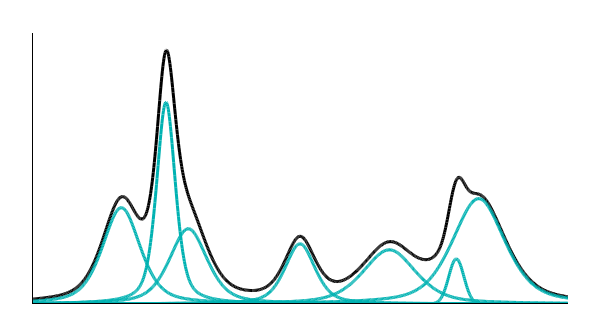
\includegraphics[width=1\linewidth]{GMM.png}
	\caption{Gaussian mixture model}
\end{figure}
The computation time for the Gaussian mixture model is more than the other methods that we experimented with. So, we modified the mixture model based on an algorithm suggested in one of the example projects \cite{proj}. The following figure outlines the steps of the algorithm.
\begin{figure}[H]\label{fch}
	\centering
	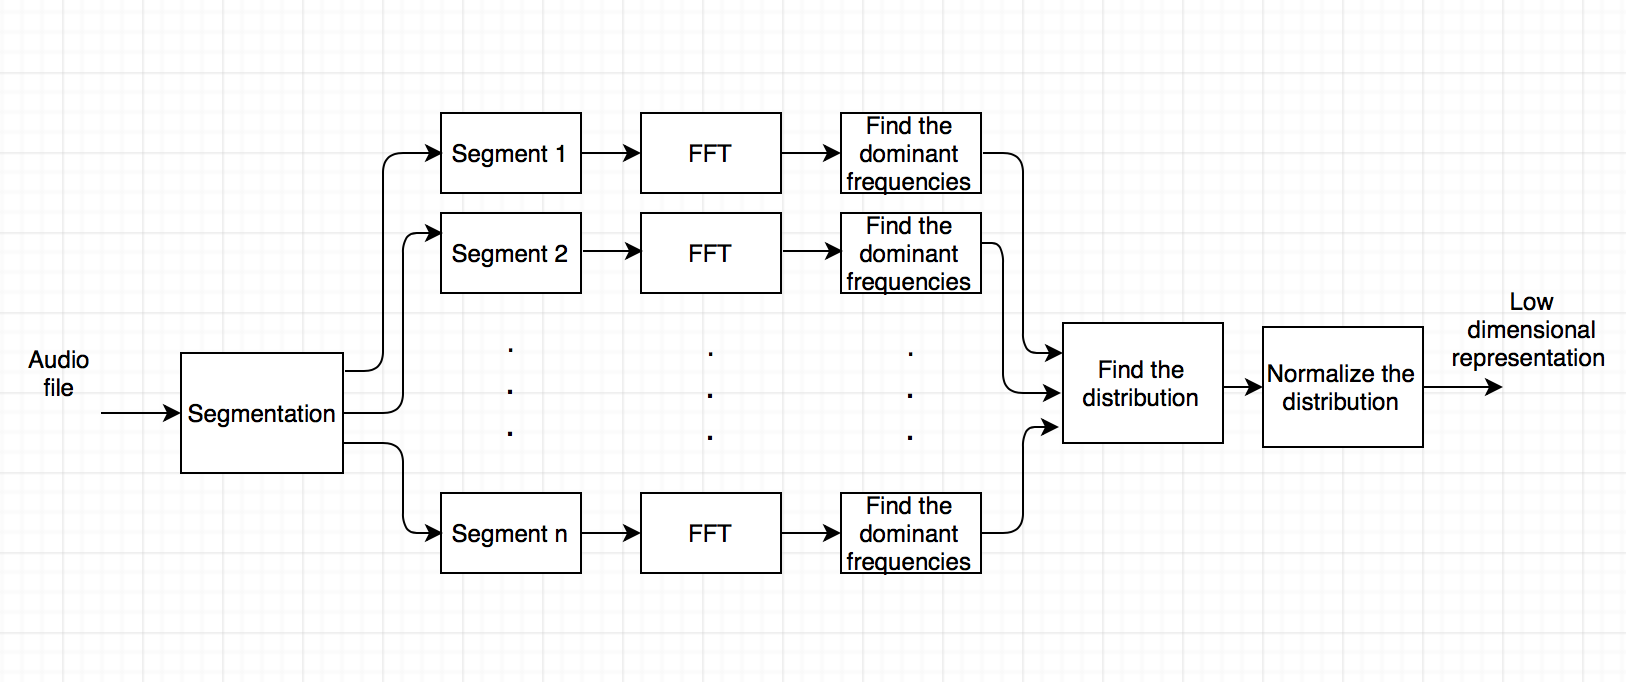
\includegraphics[width=1.1\linewidth]{fch.png}
	\caption{Modified mixture model flowchart}
\end{figure}
Based on the flowchart, we divide each song into smaller windows with the window size of 2000 samples. Then, with moving the signal to the frequency domain, we find the dominant frequency components of the signal. Repeating that for all the segments, we find the histogram of the dominant component frequency through the entire song. Since the songs have different length, we normalize the histogram by the length of each song. This distribution is the low dimension representation of the song. And, the dimension depends on the number of bins in the histogram.

\section{DISTANCE METRICS}\label{sec:dist}
This section provides the different types of distance metrics that we used in our project. Distance metric is used to quantify the distance between two different songs in the song space. However, the distance metric is valid only on a low-dimensional sub space due to curse of dimensionality. For example: Consider a hypersphere. As the number of dimension increases the volume of hypersphere tends to zero. This phenomenon is also called as concentration of measure. In such a concentrated space euclidean or any type of distance is not meaningful. Hence, before calculating the distance we need to use dimension reduction as pre-processing step. The list of techniques that we experiment with for dimension reduction is discussed in the previous section (\ref{dr}).


\subsection{MINOWSKI DISTANCE}
Minowski distance is considered as the generalization between euclidean distance and Manhattan distance. This distance metric is used along with k-nearest neighbour for classification of points for songs which was reduced by content based similarity method. The reason why we used Minowski distance over other distance metrics is based on experimentation. The distance between two n-dimensional point $ X = {x_1,x_2,...,x_n}$ and $ Y = {y_1,y_2,...,y_n} $ is calculated as:
\begin{figure}[h]\label{minowski}
\center
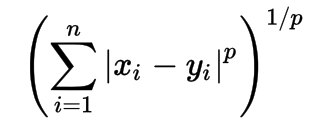
\includegraphics{fig3.png}
\caption{Minowski distance}
\end{figure}
\subsection{EARTH MOVERS DISTANCE}
Earth Movers distance is the distance between two different probability distributions over a region D. This is the distance metric used to compare the distance between two songs using the signatures generated by the content similarity method. In the field of mathematics, it is also known as wasserstein metric. Informally, it is defined as the cost of turning one pile of dirt into another. EMD value is given by the formula:
\begin{figure}[h]\label{emd}
\center
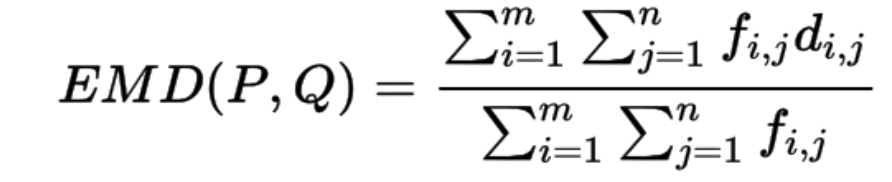
\includegraphics[scale=0.5]{emd.png}
\caption{EMD}
\end{figure}
\paragraph{}
where $f_{i,j}$ is the flow between cluster i and j and is calculated based on weight of the cluster. $d_{i,j}$ is the ground distance between the clusters. In this case euclidean distance is used as the ground distance. The numerator of the equation is denoted by the work and is normalized by the flow. The distance matrix generated by EMD is as follows:
\begin{figure}[H]\label{emd_dist}
\center
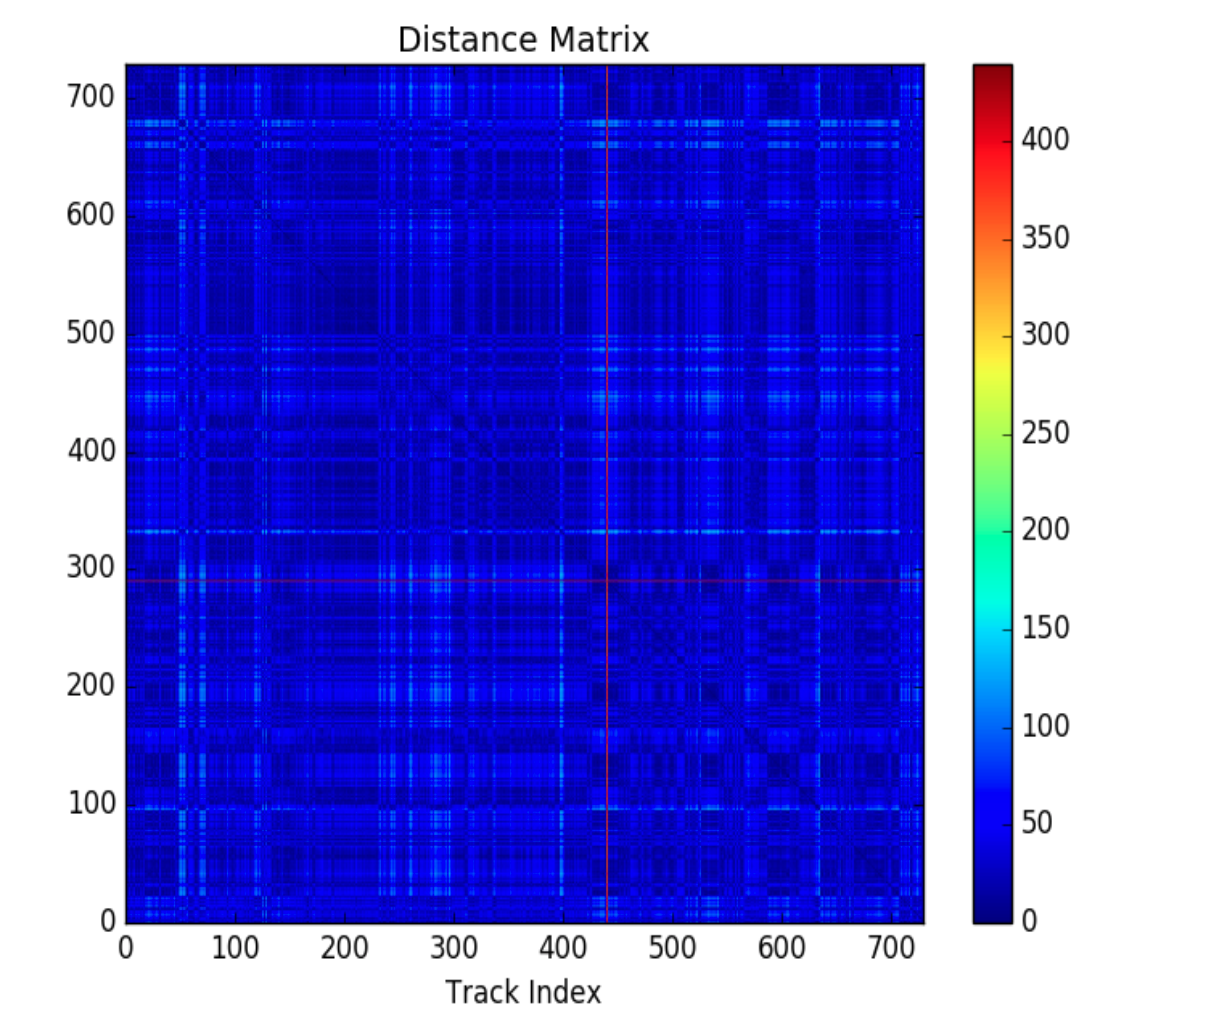
\includegraphics[scale=0.70]{emd_dist.png}
\caption{Distance matrix using EMD}
\end{figure}
In order visualize the distance matrix as scatter plot, we use multidimensional scaling (MDS). MDS is a means of visualizing the level of individual classes of a dataset. In this case, the classes refer to the different genres. Based on the scatter plot we find that there are no linearly separable regions to separate once class from another. The classes seem to be non-linearly correlated to each other. Hence, linear classification algorithms such as linear regression will not perform as expected.
\begin{figure}[H]\label{emd_scatter}
\center
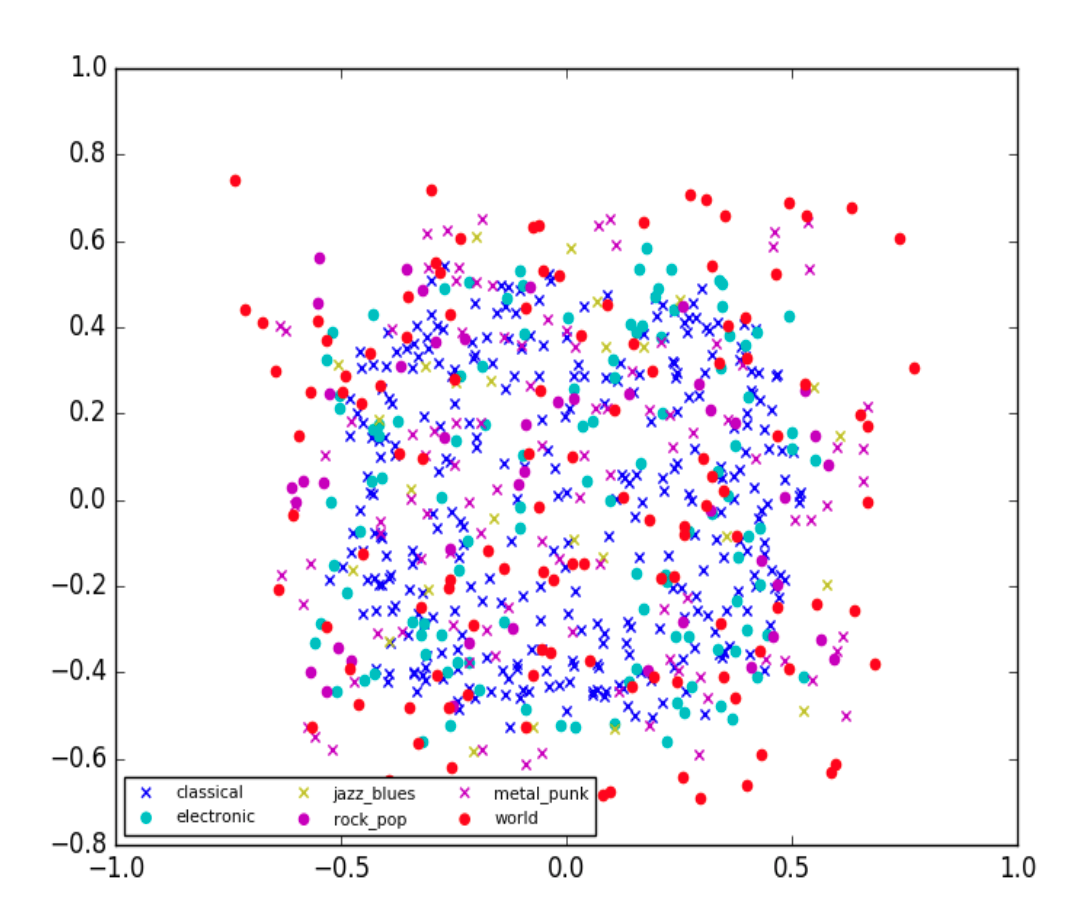
\includegraphics[scale=0.70]{emd_scatter.png}
\caption{Scatter Plot}
\end{figure}

\subsection{EUCLIDEAN DISTANCE}
Euclidean distance also known as $l^2$-norm is a common measure of distance between two points in n-dimension space. Euclidean norm is simply the magnitude of the vector. This norm is very simple to calculate. Therefore, in our experiments we start with the Euclidean norm and if the result did not provide a good performance, then we test other distance metrics relevant to the data. In addition to be simple to calculate, Euclidean distance has a good performance in a broad range of settings. The following picture represents the distance matrix using modified Gaussian mixture model and Euclidean distance.
\begin{figure}[H]\label{distMat30}
	\centering
	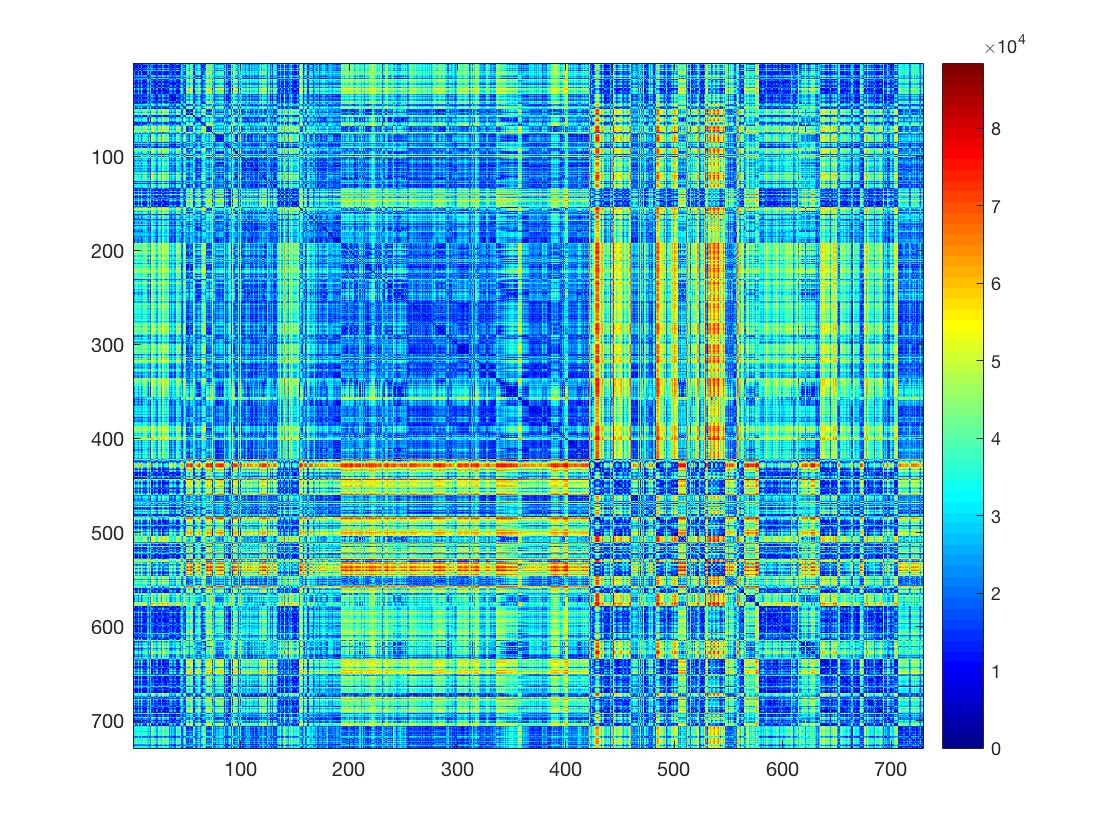
\includegraphics[width=1\linewidth]{distMat30.jpg}
	\caption{Euclidean distance matrix for modified Gaussian mixture model}
\end{figure}
We had also calculated the distance matrix using the Euclidean Distance using MFFC $\&$ PCA as well, the corresponding distance matrix is show below
\begin{figure}[H]\label{distM20}
	\centering
	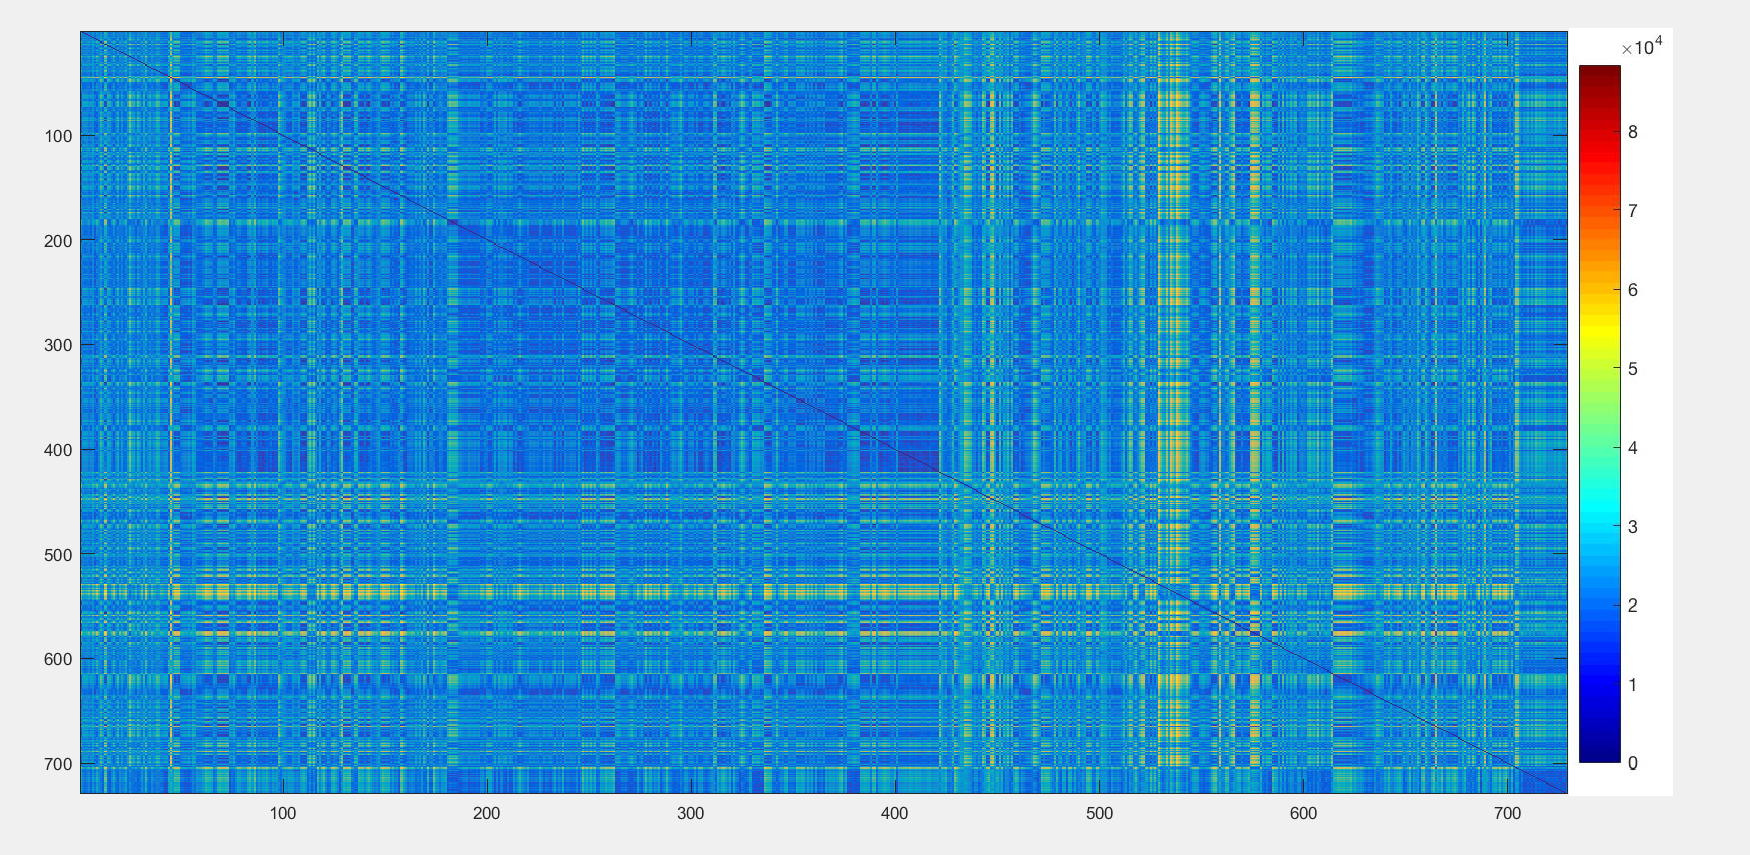
\includegraphics[width=1\linewidth]{distM20.png}
	\caption{Euclidean distance matrix for MFCC and PCA Model}
\end{figure}
\subsection{KULLBACK - LEIBLER DIVERGENCE}
Kullback-Leibler divergence (KL) distance is a measure of distance between two given probability distributions. If $P$ and $Q$ are two probability distributions, then the KL-divergence can be written as:

\begin{equation}\label{KLdist}
D_{KL}(P||Q) = H(P,Q) - H(P)
\end{equation}
In this equation, $H(P,Q)$ is the cross entropy of the two probability distributions, and $H(P)$ is the entropy of $P$. \\
For discrete probability distributions, the KL-divergence is given as the following equation:
\begin{equation}\label{KLdist}
D_{KL}(P||Q) = \sum_i P(i) log \frac{P(i)}{Q(i)}
\end{equation}
Therefore, the KL distance is a measure of the information loss in estimating probability distribution $P$ with probability distribution $Q$. As you can see from equation (\ref{KLdist}) this distance is not a symmetric distance. The following figure shows the distance matrix for our data set using modified Gaussian mixture model and KL-divergence as distance metric.
\begin{figure}[H]\label{KLDiv}
	\centering
	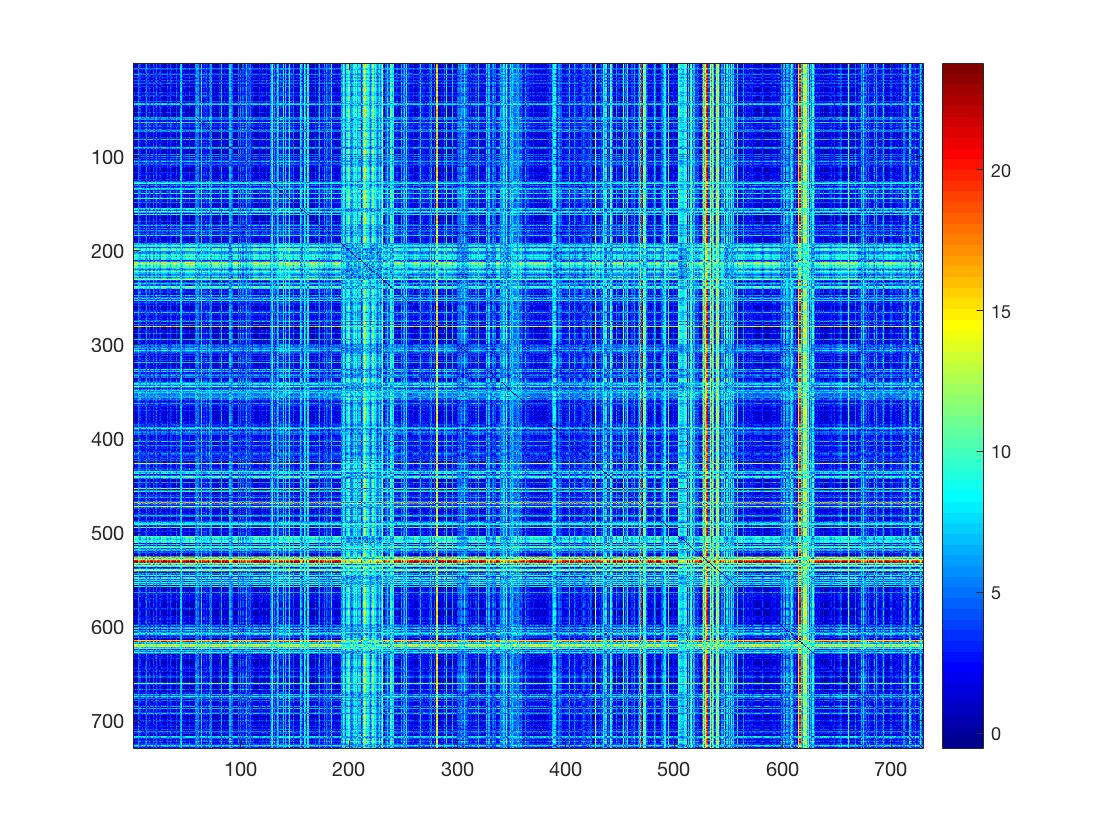
\includegraphics[width=1\linewidth]{KLDiv.jpg}
	\caption{KL distance matrix}
\end{figure}
In this distance matrix, we can see the genre classes that we have as squares around the main diagonal of the matrix. But, there is also small distance across multiple genres. For example, we can see small distance between the songs in the classical genre and the songs in the world genre.
\section{STASTICAL LEARNING}\label{sec:stat}
In previous sections we discussed the projection of audio files into lower dimensional space. And we introduced the measure of distances we use to represent the distance between the new representations of the audio files. The next step is to build the classifier to these information for genre classification. We have implemented two classification algorithms that we explain here. One of the algorithm have two different variants.
\subsection{K-NEAREST NEIGHBOURS}
One of the common algorithms for classifying multi-class data is k-nearest neighbors (kNN) \cite{li}. This algorithm simply finds the k closest data points to the testing point and determines which class owns the majority of points among these points. Therefore, the label for the testing data point would be the label of the majority of k closest data points.
The following figure represents the kNN algorithm for $k = 3$. There are 2 classes in this example represented with blue and red color. The testing point is the black circle and because 2 out of 3 closest neighbors are in blue, the classifier will assign it to the blue class.
\begin{figure}[H]\label{kNN}
	\centering
	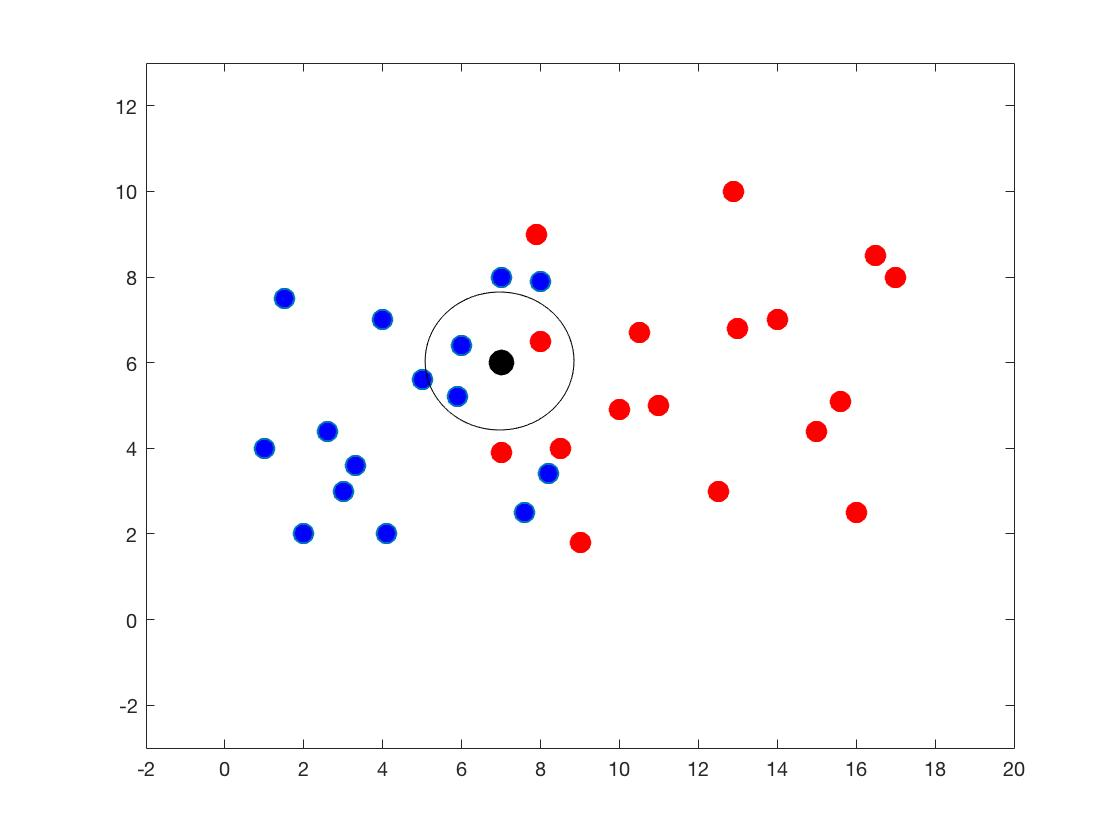
\includegraphics[width=.8\linewidth]{kNN.jpg}
	\caption{k-nearest neighbors}
\end{figure}

The kNN algorithm do not perform well as expected due to the non-uniform distribution of songs across the 6 different genres. In this project we are using 729 songs, which contains 320 classical, 115 electronics, 26 jazz-blues, 45 metal-punk, 101 rock-pop and 122 world genre. Therefore, 43\% of all songs are classical and so, in any neighborhood is more likely to have more data points from classical genre than any other genre. On the other hand, there are 26 jazz-blues songs which is less than 4\%. Thus, the probability of classifying a song as a jazz-blues song using kNN classifier is very low. Therefore, the kNN does not provide a good performance for the data set that we are using. The major error using kNN is classifying non-classical songs as classical songs. It also has a 100\% error for jazz-blues genre. In order to overcome this problem we have modified the kNN algorithm to take into account the frequency of each genre.

\subsection{MODIFIED K-NN}
As we mentioned in the previous section, in order to make kNN classifier more powerful we introduced the modified kNN algorithm. In the modified-kNN classifier, we normalize the number of neighbors in each genre by the frequency of that genre (the number of training points in that genre divided by the total number of training points) in the training data. This classifier can be considered a special case of weighted-kNN, where the weights are the frequency of that genre. This algorithm improves the results for genres other than classical genre, but degrades the performance for the classical genre. And, the overall accuracy of the classifier increases.

\subsection{NEURAL NETWORK}
Neural network is a machine learning algorithm that is inspired from the biological brain. it is amazing how different neurons in the brain wire and fire together in order to accomplish various tasks in our every day life.
The neural architecture that we incorporate in this project is based on  feedforward-back propagation algorithm.
The neural network basically consist of three different layers
\begin{itemize}
  \item Input layer
  \item Hidden layer
   \item Output layer
\end{itemize}

The diagram below shows the different layers of a sample neural network.
\begin{figure}[H]
\center
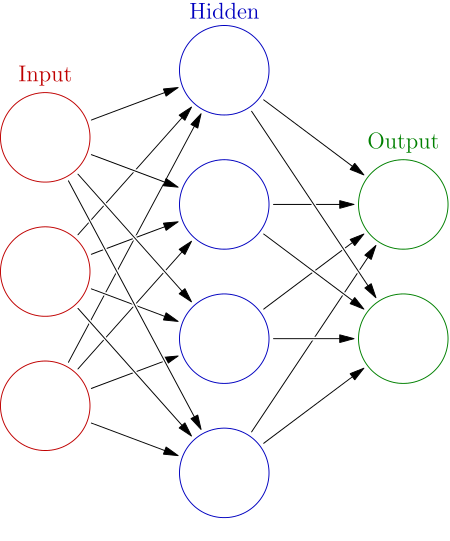
\includegraphics [scale=0.5]{ann.png}
\caption{Sample Neural Network}
\end{figure}
The connections between the input Layer and the hidden layer have weights that are multiplied to each connection. The weights are selected as per Gaussian values i.e they are between 0 and 1.
The Hidden Layer also have an active function which could be any mathematical function. For our classification we have used Levenberg-Marquardt


The neural network has three contributing factor that changes the efficiency of the output.
\begin{itemize}
  \item Weights given to the connections
  \item Active function of the hidden layer
   \item The Learning algorithm
   \end{itemize}
The learning algorithm used is back propagation. The difference between the expected and actual output is calculated and fed back into the network in order to update the synaptic weights. Over time, the difference or error reduces and the neural network will be able to learn the task.\\
 The neural network used in this project is shown below
\begin{figure}[H]
\center
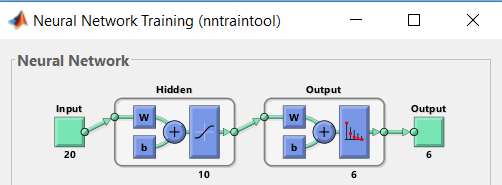
\includegraphics [scale=0.5]{neuralnet.png}
\caption{Neural network model}
\end{figure}
The input given is 20 features for each song and this is passed to hidden layer that contains 10 neurons and finally classifies the input to 6 genres.

\section{EXPERIMENTS}\label{sec:exp}
%_________________________________________________________________
The general idea for genre classification is first Dimensionality Reduction, finding the distance matrix and then classifying the genres.
Hence in this project we used various dimensionality reductions such as MFCC,PCA,modified gaussian mixture model and Content based similarity. Decreasing the dimension is a crucial in genre classification as it avoids dimensionality curse.
In this project we tried a different set of combinations of the dimensionality reduction,distance calculation and classification methods.
The distance matrix is calculated for all the methods.\\
The confusion matrix for all the methods are shown below. First is the result of the Signature method (content based similarity) Dimensionality reduction for which the distance is calculated through Earth mover distance method and classified into genre using KNN Classification.
\begin{figure}[H]
\center
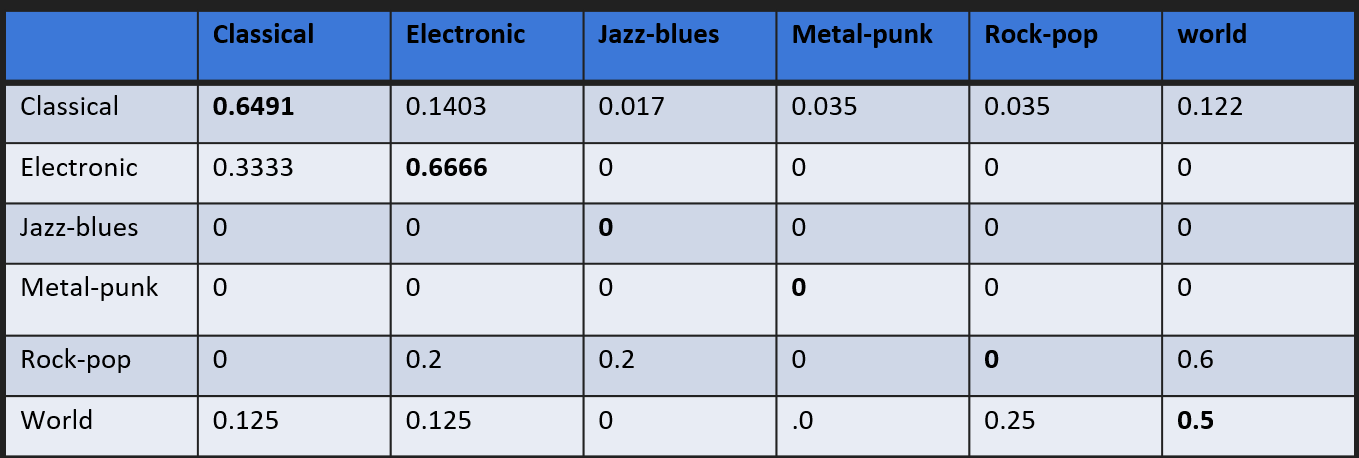
\includegraphics [scale=0.35]{results1.png}
\caption{Confusion Matrix for Content based similarity approach}
\end{figure}
The average accuracy for this method was 54. \\
The second method that was performed was using Modified Gaussian mixture with euclidean distance and KNN classification.The efficiency obtained for this method is $52$.
\begin{figure}[H]
\center
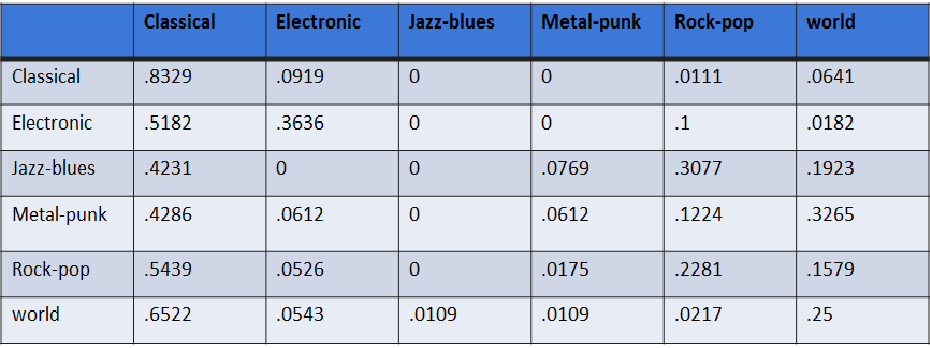
\includegraphics [scale=0.65]{result2.png}
\caption{Confusion Matrix for Gaussian mixture and KNN d=20 }
\end{figure}
We tried increasing the dimension and performed the same methods as above we can say that the efficiency increases as the dimensions are increased. Below is the confusion matrix when d=50.
\begin{figure}[H]
\center
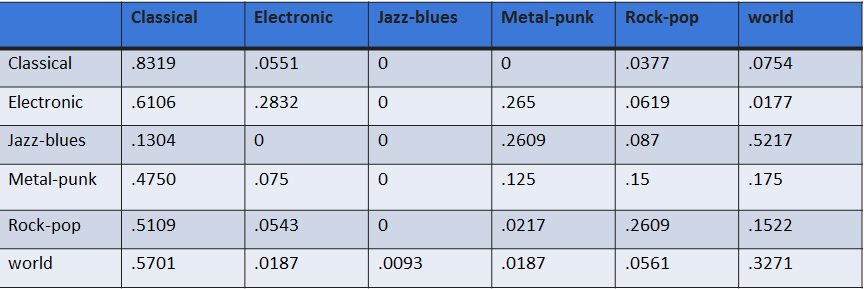
\includegraphics [scale=0.7]{result3.png}
\caption{Confusion Matrix for Gaussian mixture and KNN d=50 }
\end{figure}
Next we changed the method by which the classification to obtain better classification of genre.Modified KNN method was used which gave better results as shown in the confusion matrix below.
\begin{figure}[H]
\center
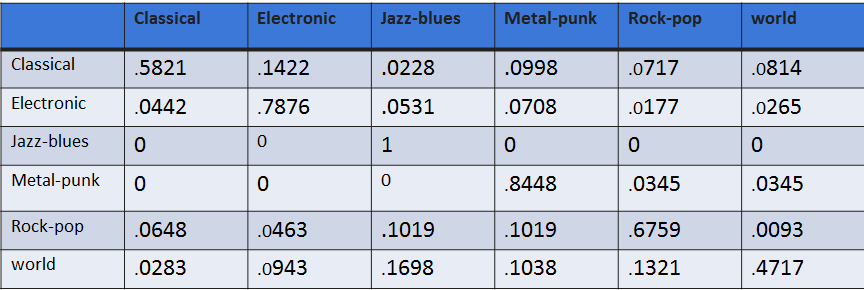
\includegraphics [scale=0.7]{result4.png}
\caption{Confusion Matrix for Gaussian mixture and Modified KNN d=50 }
\end{figure}
Finally the basic method of dimensionality reduction was implemented a(MFCC and PCA),euclidean distance and neural network method of classification was performed.
\begin{figure}[H]
\center
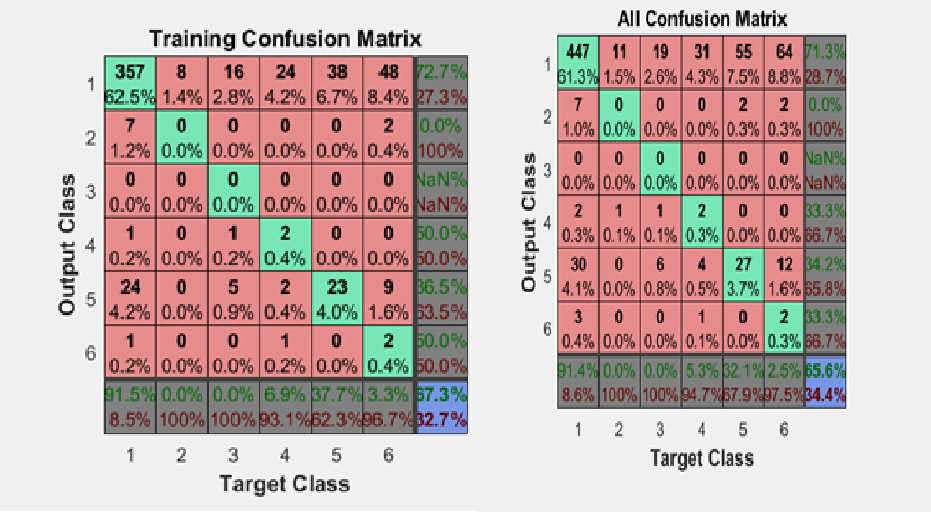
\includegraphics [scale=0.7]{result5.png}
\caption{Confusion Matrix for Neural network }
\end{figure}
The input given Below is the table that shows the combination of methods we tried and their result.
\begin{figure}[H]
\center
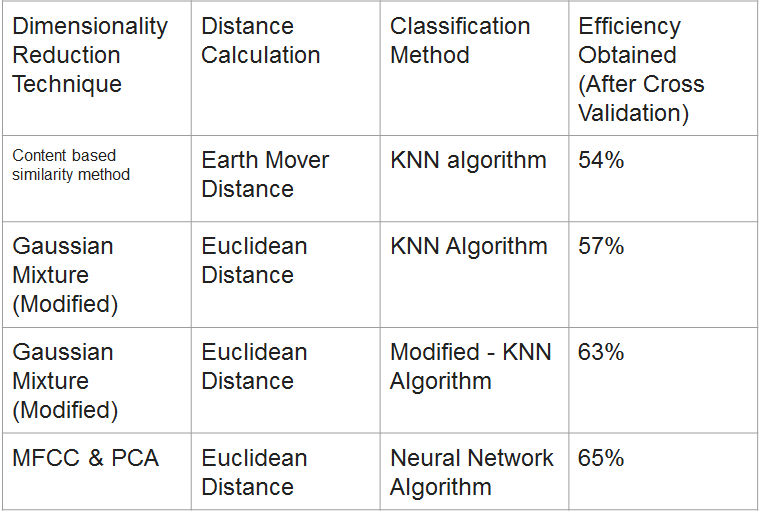
\includegraphics [scale=0.7]{table.png}
\caption{Summary}
\end{figure}
We could say that our algorithms for genre classification worked fairly. If we had randomly classified our input data into classical and non-classical we would have got 50$\%$ accuracy. All our algorithm gave us more than $50\%$ efficiency with 6 genre classification.
The computation time for running all,these programs were long as we had to sample and reduce dimension for 729 songs.Though Gaussian mixture model gave us the fastest results among all three.
%_________________________________________________________________
\section{DISCUSSION}\label{sec:disc}
Music genre classification is a hard task. Our approach is three fold: Apply dimension reduction, calculate distance matrix and classify the data into its corresponding genres. For each stage, we experimented with different algorithms in an effort to achieve better accuracy across individual genres as well as overall accuracy.One of the important challenge that we encountered was the distribution of the data. The dataset has proportionately more classical songs than the other genres such as jazz or rock pop. This bias led to higher accuracy in classical and bad performance across another genres. As a solution we tried implementing modified k-nearest neighbours. Although, the accuracy improved from 57$\%$ to 63$\%$, the accuracy across classical dropped while the accuracy increased across other genres.

\paragraph{}
As the next steps, we would like to try extracting features such as rhythm, modulation, amplification and other parameters instead of just the raw signal \cite{tzan} \cite{lee}. In addition, we are interested in studying the performance of the algorithm across different possible distance metrics. For example: In content based similarity dimensionality reduction, we use k-Means along with euclidean distance to cluster. How would it differ if we used Kullback Leibler instead of euclidean?. With respect of neural networks we would like to try different learning algorithms such as particle swarm optimization in order to find the synaptic weights of the network \cite{gudise}. Overall, the next steps would focus on improving the accuracy across genres as well as the overall accuracy.
\begin{thebibliography}{9}
	\bibitem{logan}\label{logan}
	Logan, B., & Salomon, A. (2001). A content-based music similarity function. Cambridge Research Labs-Tech Report.
	\bibitem{pampalk}\label{pampalk}
	Pampalk, E. (2006). Computational models of music similarity and their application in music information retrieval. na.
	\bibitem{lee}
	Lee, C. H., Shih, J. L., Yu, K. M., & Lin, H. S. (2009). Automatic music genre classification based on modulation spectral analysis of spectral and cepstral features. IEEE Transactions on Multimedia, 11(4), 670-682.
	\bibitem{tzan}
	Tzanetakis, George, and Perry Cook. "Musical genre classification of audio signals." IEEE Transactions on speech and audio processing 10.5 (2002): 293-302.
	\bibitem{holand}
	Holand, S. M. (2008). Principal components analysis (PCA). Department of Geology, University of Georgia, Athens, GA.
	\bibitem{logmfcc}
	Logan, B. (2000, October). Mel Frequency Cepstral Coefficients for Music Modeling. In ISMIR.
	\bibitem{li}
	Li, T., Ogihara, M., & Li, Q. (2003, July). A comparative study on content-based music genre classification. In Proceedings of the 26th annual international ACM SIGIR conference on Research and development in informaion retrieval (pp. 282-289). ACM.
	\bibitem{dasgupta}
	Dasgupta, S., & Gupta, A. (2003). An elementary proof of a theorem of Johnson and Lindenstrauss. Random Structures & Algorithms, 22(1), 60-65.
	\bibitem{gudise}
	Gudise, V. G., & Venayagamoorthy, G. K. (2003, April). Comparison of particle swarm optimization and backpropagation as training algorithms for neural networks. In Swarm Intelligence Symposium, 2003. SIS'03. Proceedings of the 2003 IEEE (pp. 110-117). IEEE.
	\bibitem{proj}
	http://ecee.colorado.edu/~fmeyer/class/ecen5322/example2.pdf
\end{thebibliography}
\end{document}